\documentclass[12pt]{article}

% UTF-8 encoding and fonts
\usepackage[utf8]{inputenc}
\usepackage[T1]{fontenc}
\usepackage{lmodern}

% Page setup
\usepackage[margin=1in]{geometry}
\usepackage{setspace}
\onehalfspacing

% Math and symbols
\usepackage{amsmath,amssymb}

% Graphics
\usepackage{graphicx}
\usepackage{float}
\usepackage{tikz}
\usepackage{pgfplots}
\pgfplotsset{compat=1.17}

% Tables
\usepackage{booktabs}
\usepackage{array}
\usepackage{multirow}
\usepackage{threeparttable}

% Bibliography
\usepackage{natbib}
\bibliographystyle{plainnat}

% Hyperlinks
\usepackage{hyperref}
\hypersetup{
    colorlinks=true,
    linkcolor=blue,
    citecolor=blue,
    urlcolor=blue
}

% Captions
\usepackage{caption}
\captionsetup{font=small,labelfont=bf}

% Section formatting
\usepackage{titlesec}
\titleformat{\section}{\large\bfseries}{\thesection.}{0.5em}{}
\titleformat{\subsection}{\normalsize\bfseries}{\thesubsection}{0.5em}{}

% Custom commands
\newcommand{\E}{\mathbb{E}}
\newcommand{\Var}{\text{Var}}
\newcommand{\Cov}{\text{Cov}}

% APEP Working Paper formatting
\title{Does Colorado's Old Age Pension Reduce Labor Supply? \\ Evidence from a Regression Discontinuity Design}
\author{APEP Autonomous Research\thanks{%
Autonomous Policy Evaluation Project.
This paper was autonomously generated using Claude Code.
Contributor: CONTRIBUTOR\_GITHUB.
Repository: github.com/dakoyana/auto-policy-evals Contributor: @dakoyana.}}
\date{January 2026}

\begin{document}

\maketitle

\begin{abstract}
\noindent
Colorado's Old Age Pension (OAP) program, established in the state constitution in 1937, provides cash benefits to low-income residents beginning at age 60---five years earlier than most comparable programs. This unique age threshold creates a potential regression discontinuity design for studying labor supply effects of early retirement benefits. Using American Community Survey microdata from 2015--2023, I examine whether crossing the age-60 eligibility threshold affects labor force participation among low-income Coloradans. The primary analysis finds no statistically significant discontinuity in labor force participation at age 60 among low-income individuals (effect: $-1.7$ percentage points, SE: $1.5$ pp). The weak first stage---public assistance receipt shows no discontinuous jump at age 60---suggests limited program take-up among the eligible population. Placebo tests reveal significant effects at non-threshold ages, indicating that age-related labor force exit in this population follows a smooth decline rather than a sharp discontinuity at 60. Exploratory heterogeneity analysis suggests larger effects among college-educated low-income individuals ($-7.3$ pp, significant), though this finding requires cautious interpretation given the lack of pre-registration. These results highlight the challenge of identifying program-specific effects when take-up is limited and underscore the importance of first-stage verification in RDD studies of social insurance programs.
\end{abstract}

\vspace{1em}
\noindent\textbf{JEL Codes:} H55, J22, J26 \\
\noindent\textbf{Keywords:} old age pension, labor supply, regression discontinuity, Colorado, social insurance

\newpage

%==============================================================================
\section{Introduction}
%==============================================================================

Understanding how social insurance programs affect labor supply decisions is a central question in public economics. Government transfers to older adults, whether through Social Security, Supplemental Security Income, or state-level pension programs, may reduce work incentives by providing non-labor income and, in many cases, imposing implicit taxes on earnings through means-testing. The magnitude of these labor supply responses has important implications for program design, fiscal sustainability, and the welfare of older workers who may face declining productivity or health limitations. As populations age across developed economies, understanding these behavioral responses becomes increasingly important for designing sustainable social insurance systems.

The theoretical predictions about labor supply responses to old-age benefits are clear. Standard economic theory suggests that cash transfers create income effects that reduce labor supply when leisure is a normal good. Beyond this income effect, means-tested programs create implicit marginal taxes on earnings: each dollar earned may reduce benefits by some fraction, effectively taxing work at high rates. When means-testing is particularly stringent---as when benefits are reduced dollar-for-dollar with earnings---the implicit marginal tax rate can reach 100 percent, creating powerful disincentives for formal employment. These theoretical predictions have been extensively documented in empirical work, though the magnitudes vary considerably across programs and settings.

This paper investigates whether Colorado's Old Age Pension (OAP) program affects labor force participation among low-income older adults. The OAP is a distinctive program: established in the Colorado state constitution in 1937, it provides monthly cash benefits to residents aged 60 and older with limited income and assets. This age threshold is notably earlier than the age-65 eligibility for Medicare and the full retirement age for Social Security, making it one of the earliest state-level cash assistance programs for older adults in the United States. The constitutional status of the program has provided unusual stability over nearly nine decades, avoiding the frequent legislative changes that complicate analysis of many social programs. The sharp age-60 cutoff creates a natural setting for regression discontinuity analysis, as individuals just below and just above the threshold should be similar in all respects except for OAP eligibility.

I use individual-level microdata from the American Community Survey (ACS) Public Use Microdata Sample for 2015--2023 to estimate the effect of OAP eligibility on labor force participation. The research design compares labor market outcomes for individuals just below age 60 to those just above, exploiting the discontinuous change in eligibility status at this threshold. To focus on the population most likely affected by the program, I restrict the primary analysis to low-income individuals whose total personal income falls below \$20,000 annually. This targeting is essential because the OAP is means-tested, and higher-income individuals would be ineligible regardless of age.

The main findings of this study are largely null. Among low-income Colorado residents aged 55--65, labor force participation shows no statistically significant discontinuity at age 60: the point estimate is $-1.7$ percentage points with a standard error of 1.5 percentage points (t-statistic: $-1.1$). This estimate is small relative to the baseline labor force participation rate of 28 percent in this sample and cannot be distinguished from zero at conventional significance levels. The 95 percent confidence interval ranges from approximately $-4.6$ to $+1.2$ percentage points, ruling out large negative effects but unable to distinguish modest effects from zero. The lack of a detectable effect persists across bandwidth specifications and alternative sample definitions, suggesting the null finding is robust to methodological choices.

Several validity checks raise concerns about the ability of this design to isolate OAP-specific effects. Most critically, the first stage is weak: public assistance income---the closest proxy for OAP receipt available in the ACS---shows no discontinuous increase at age 60. Among low-income individuals, the probability of receiving any public assistance changes by only 0.03 percentage points at the threshold, with a standard error of 0.59 percentage points. This null first stage suggests that either program take-up is limited among eligible individuals, the ACS's public assistance variable does not adequately capture OAP receipt, or both. Without a strong first stage, reduced-form estimates cannot be confidently interpreted as program effects.

Placebo tests at non-threshold ages (58 and 62) reveal statistically significant effects comparable in magnitude to those observed at age 60, indicating that labor force exit in this population follows a smooth age-related decline rather than a sharp discontinuity at any particular age. The placebo estimate at age 58 is $-4.9$ percentage points (significant at the 1 percent level), and the estimate at age 62 is $-4.7$ percentage points (also highly significant). These patterns suggest that detecting discontinuities in this population is difficult when the underlying process is continuous but the running variable---age in integer years---is discrete. Any age-specific estimate must be interpreted against this backdrop of general age-related decline.

Exploratory heterogeneity analysis reveals one intriguing pattern: among college-educated low-income individuals, the discontinuity at age 60 is larger and statistically significant ($-7.3$ percentage points, SE: 2.6 pp, t-statistic: $-2.76$). This subgroup effect was not pre-specified and should be interpreted cautiously. It could reflect genuine heterogeneity in program awareness or responsiveness among more educated individuals, who may be better able to navigate bureaucratic application processes or may have stronger preferences for early retirement. Alternatively, it could be a spurious finding arising from multiple testing---examining many subgroups increases the probability of finding at least one significant result by chance.

This paper contributes to several literatures. First, it adds to the large body of research on how social insurance programs affect labor supply at older ages. The seminal work of \citet{gruber_disability_1998} on Canadian disability insurance demonstrated substantial labor supply responses to benefit availability. \citet{autor_rise_2003} documented similar patterns in the United States, finding that the expansion of disability insurance contributed meaningfully to declining labor force participation among working-age adults. Studies of Social Security have found meaningful responses to eligibility ages and benefit levels \citep{french_effects_2011, manoli_nonparametric_2016, mastrobuoni_labor_2009}. More recently, \citet{fetter_government_2018} used historical data on Old Age Assistance programs in the 1940s to show that these early pension programs reduced labor force participation by approximately 8.5 percentage points among men aged 65--74. My study examines a modern analogue of these programs, though the null findings suggest that either the institutional setting differs importantly or measurement challenges in contemporary survey data make detection difficult.

Second, this paper contributes to the growing literature using regression discontinuity designs to study age-based policy thresholds. Following the methodological contributions of \citet{imbens_regression_2008} and \citet{lee_regression_2010}, researchers have exploited age discontinuities in Medicare eligibility \citep{card_does_2008, card_medicare_2009}, Social Security benefits \citep{gelber_effects_2017}, minimum wage provisions \citep{cahuc_youth_2019}, and health insurance access \citep{sommers_changes_2012}. A key lesson from this literature is the importance of first-stage verification: RDD estimates are only informative about program effects when the threshold actually induces a meaningful change in treatment status. The weak first stage in my analysis underscores this point and contributes to understanding the limitations of RDD designs when take-up is incomplete.

Third, this paper provides new evidence on a relatively understudied state-level program. While federal programs like Social Security and Medicare have been extensively analyzed, state-level variation in safety net generosity has received less attention, particularly for programs targeting older adults. Colorado's OAP is unusual in its constitutional status and early eligibility age, making it a distinctive case for understanding how institutional features of social insurance affect behavior. The null findings contribute to a growing literature documenting the challenges of identifying program effects in settings with limited take-up \citep{currie_take_2006, moffitt_welfare_1983}.

The remainder of this paper proceeds as follows. Section 2 describes the institutional background of Colorado's Old Age Pension program. Section 3 reviews the related literature on social insurance and labor supply. Section 4 presents a simple theoretical framework. Section 5 describes the data and sample construction. Section 6 presents the empirical strategy. Section 7 reports the main results and validity checks. Section 8 presents robustness and heterogeneity analyses. Section 9 discusses the findings and their implications, and Section 10 concludes.

%==============================================================================
\section{Institutional Background}
%==============================================================================

Colorado's Old Age Pension program has a distinctive history and institutional structure that make it unusual among state-level assistance programs. Understanding these features is essential for interpreting the empirical analysis and assessing the external validity of the findings.

\subsection{Historical Origins}

The OAP was established through a constitutional amendment approved by Colorado voters in 1936 and implemented beginning in 1937. This timing is significant: the program predates the widespread implementation of Social Security (which began paying benefits in 1940) and represents one of the earliest state-level responses to old-age poverty during the Great Depression. The economic crisis of the 1930s created widespread destitution among older Americans, many of whom had seen their savings wiped out by bank failures and had no means of support. States across the country experimented with various forms of old-age assistance during this period, though most of these programs were later absorbed into or superseded by federal programs.

Unlike many other state programs from this era, the OAP remains enshrined in the Colorado constitution and continues to operate as a distinct state program. The constitutional status has important implications: it cannot be easily modified by the state legislature and has provided unusual stability over nearly nine decades. While benefit levels and administrative details have changed over time, the fundamental structure of the program---including the age-60 eligibility threshold---has remained consistent.

\subsection{Eligibility Requirements}

The most distinctive feature of the OAP is its age threshold. While federal programs like Supplemental Security Income require recipients to be aged 65 or older (or disabled), and while Social Security benefits are available beginning at age 62, the OAP provides benefits to Colorado residents beginning at age 60. This five-year difference from the more common age-65 threshold creates a unique policy environment in which Coloradans become eligible for cash assistance earlier than residents of most other states.

Program eligibility requires meeting several criteria beyond the age requirement. First, applicants must be legal residents of Colorado. Second, they must meet income tests designed to target benefits to low-income individuals. The income test considers all sources of income, including wages, Social Security, pensions, and any other regular income. Third, applicants must meet asset tests that limit countable resources, though the primary residence is generally excluded from this calculation. These means-testing provisions ensure that the program targets assistance to those with limited alternative resources.

\subsection{Benefit Structure}

The benefit structure provides a guaranteed minimum income level. As of 2026, the maximum monthly OAP benefit is approximately \$1,032, though this amount is reduced for individuals with other income sources. Specifically, benefits are reduced dollar-for-dollar for income above a minimal threshold, creating an implicit 100 percent marginal tax rate on earnings for beneficiaries. This feature of the program is central to understanding its potential labor supply effects: each dollar earned reduces benefits by a dollar, eliminating any financial gain from working for those receiving full benefits.

The program thus functions as a safety net that tops up income to a specified floor, similar in structure to SSI but with an earlier eligibility age. The guaranteed income level has been adjusted periodically to reflect cost-of-living changes, though it remains modest by contemporary standards. For individuals with no other income, the OAP provides basic subsistence support but not financial security.

\subsection{OAP Health Care Benefits}

The OAP Health Care Program (OAP-B) provides additional benefits for recipients aged 60--64 who are not yet eligible for Medicare. This health coverage component may further enhance the value of the program for pre-65 recipients. Health insurance access is particularly valuable for this age group, who often face high premiums in the individual insurance market and may have pre-existing conditions that historically limited coverage options. The health benefit adds to the total value of becoming OAP-eligible at age 60, potentially strengthening any labor supply response.

\subsection{Implications for Research Design}

Several features of the OAP are relevant for the empirical analysis. First, the sharp age-60 threshold creates a discontinuity in eligibility that can potentially be exploited for causal identification. Individuals just below 60 are categorically ineligible regardless of their income, while those just above may qualify if they meet the other criteria. This sharp cutoff is ideal for regression discontinuity analysis.

Second, the dollar-for-dollar benefit reduction creates strong theoretical predictions about labor supply: economic theory suggests that the income effect from the transfer should reduce labor supply, while the implicit marginal tax should create additional disincentives for work among beneficiaries. The combination of these effects suggests we should observe reduced labor force participation among program recipients.

Third, the constitutional status of the program means it has remained relatively stable over time, avoiding the frequent policy changes that complicate analysis of some federal programs. This stability allows pooling multiple years of data without concern about changing program rules confounding the estimates.

However, several challenges complicate the analysis. The OAP is not directly identifiable in the American Community Survey data used in this study. The ACS asks about ``public assistance income,'' which may include OAP benefits but also captures other programs like Temporary Assistance for Needy Families. This measurement limitation means the first stage---the relationship between crossing age 60 and receiving OAP benefits---must be inferred rather than directly observed. Additionally, program take-up may be incomplete due to lack of awareness, stigma, or transaction costs associated with applying.

%==============================================================================
\section{Related Literature}
%==============================================================================

This paper relates to several strands of the economics literature on social insurance, labor supply, and regression discontinuity methods. I review each in turn, highlighting connections to the current study.

\subsection{Social Insurance and Labor Supply at Older Ages}

A central question in public economics concerns how social insurance programs affect work decisions. The theoretical framework is straightforward: cash transfers provide income that substitutes for earnings, while means-testing creates implicit taxes on work. Both channels predict reductions in labor supply among program beneficiaries or those eligible for benefits. The empirical challenge lies in isolating causal effects from selection---individuals who take up benefits may differ from non-recipients in unobserved ways that also affect their labor supply.

The empirical literature has generally confirmed theoretical predictions, though with considerable variation in estimated magnitudes across programs and settings. \citet{gruber_disability_1998} showed that disability insurance programs in Canada induced substantial labor force exit, with a 10 percent increase in benefits reducing labor force participation by approximately 3 percentage points. This work demonstrated that social insurance can have meaningful effects on work decisions even among populations that face genuine health limitations.

\citet{autor_rise_2003} documented similar patterns in the United States, finding that the expansion of disability insurance contributed meaningfully to declining labor force participation among working-age adults. Their work highlighted the importance of screening strictness---as disability determination became more lenient, more individuals with marginal impairments chose to claim benefits rather than continue working. This finding has important implications for program design, suggesting that the structure of eligibility determination affects behavioral responses.

Studies focusing specifically on older workers have found significant responses to Social Security provisions. \citet{french_effects_2011} estimated a structural model of retirement and found that eliminating the Social Security earnings test would substantially increase labor supply among beneficiaries. The earnings test, which reduces benefits for those who work while receiving Social Security before full retirement age, creates implicit marginal tax rates that discourage work. \citet{manoli_nonparametric_2016} used bunching methods to estimate labor supply responses to Social Security rules, finding meaningful elasticities that imply workers actively adjust their behavior in response to program incentives.

\citet{mastrobuoni_labor_2009} examined the effects of changes in Social Security's full retirement age, finding that workers respond to these policy parameters by adjusting their retirement timing. This work demonstrated that even relatively small changes in incentives can affect behavior when workers are near the margin of retirement decisions. \citet{coile_social_2007} provided comprehensive evidence on how Social Security wealth and accrual rates affect retirement timing, finding substantial responses to program incentives.

Most directly relevant to this paper, \citet{fetter_government_2018} studied the labor supply effects of Old Age Assistance programs in the 1940s using the large variation in program generosity across states. Their regression discontinuity estimates suggest that OAA reduced labor force participation among men aged 65--74 by 8.5 percentage points, accounting for more than half of the decline in late-life work between 1930 and 1940. Their findings demonstrate that early pension programs had substantial effects on work behavior, though the historical context differs importantly from the contemporary setting I examine.

\subsection{Incomplete Take-up of Social Programs}

A large literature documents that take-up of means-tested social programs is often incomplete, with substantial shares of eligible individuals not receiving benefits. \citet{currie_take_2006} reviewed this evidence across multiple programs, finding take-up rates ranging from approximately 50 to 80 percent for most means-tested programs. Low take-up can arise from several factors: lack of information about program existence or eligibility, stigma associated with receiving benefits, transaction costs of applying, or strategic decisions to preserve future eligibility.

\citet{moffitt_welfare_1983} developed an influential model of stigma effects in welfare participation, showing that aversion to receiving government benefits can explain low take-up even when financial benefits would be substantial. \citet{kleven_unwilling_2011} documented similar patterns in Denmark, finding that information interventions could increase take-up of retirement benefits. These findings suggest that observed take-up rates understate potential program effects on behavior---if more eligible individuals claimed benefits, labor supply effects could be larger.

The incomplete take-up literature has important implications for my analysis. If OAP take-up is low, the first stage of the RDD design will be weak, and reduced-form estimates will understate the effect of actually receiving benefits on those who would receive them. The null findings in this paper could reflect genuinely small effects or could reflect measurement challenges arising from limited take-up.

\subsection{Regression Discontinuity Methods}

The regression discontinuity design has become a workhorse method for causal inference in economics since its revival by \citet{angrist_identification_1999} and subsequent methodological development. The foundational contributions of \citet{imbens_regression_2008} and \citet{lee_regression_2010} established best practices for implementation and interpretation. Key requirements include the continuity of potential outcomes at the threshold (which rules out sorting or manipulation) and sufficient variation in the running variable to estimate effects at the cutoff.

Age-based discontinuities have been particularly valuable because age is difficult to manipulate and progresses uniformly. \citet{card_does_2008} exploited the Medicare eligibility threshold at age 65 to study effects on health care utilization and health outcomes. \citet{card_medicare_2009} extended this analysis to examine effects on mortality, finding that Medicare eligibility substantially increased access to care. \citet{gelber_effects_2017} used the Social Security earnings test threshold to estimate labor supply elasticities. These studies demonstrate the power of age-based RDD but also highlight the challenge of isolating specific program effects when multiple policies share the same threshold.

\citet{sommers_changes_2012} used the age-26 threshold for dependent coverage under the Affordable Care Act to study effects on insurance coverage and health care access, demonstrating how age-based policies can be evaluated using RDD methods. \citet{cahuc_youth_2019} studied age-based minimum wage provisions in France, finding effects on employment and school enrollment.

A key lesson from this literature is the importance of first-stage verification in ``fuzzy'' RDD settings where the threshold affects treatment probability rather than guaranteeing treatment. Without evidence that crossing the threshold actually changes treatment status, reduced-form estimates are difficult to interpret as program effects.

%==============================================================================
\section{Theoretical Framework}
%==============================================================================

This section develops a simple theoretical framework to guide the empirical analysis and interpretation of results. The framework highlights the channels through which OAP eligibility might affect labor supply and generates testable predictions.

\subsection{Basic Setup}

Consider an individual who makes labor supply decisions to maximize utility from consumption and leisure. Let $U(c, l)$ denote utility, where $c$ is consumption and $l$ is leisure. The individual has a time endowment $T$ that can be allocated between leisure and work ($h = T - l$), earning wage $w$ per hour worked. Total income is $y = wh + n$, where $n$ represents non-labor income.

In the absence of the OAP, the individual solves:
\begin{equation}
\max_{h} U(wh + n, T - h) \text{ subject to } h \geq 0
\end{equation}

The optimal labor supply $h^*(w, n)$ depends on the wage rate and non-labor income. Standard assumptions imply that $\partial h^* / \partial n < 0$ when leisure is a normal good---increases in non-labor income reduce labor supply.

\subsection{Introducing the OAP}

The OAP introduces a transfer $B$ to eligible individuals, but this transfer is reduced dollar-for-dollar with earnings. Let $B_0$ denote the maximum benefit level. If the individual works and earns $wh$, the actual benefit received is:
\begin{equation}
B(h) = \max\{B_0 - wh, 0\}
\end{equation}

Total income under the OAP is therefore:
\begin{equation}
y = wh + n + \max\{B_0 - wh, 0\} = \max\{wh + n, B_0 + n\}
\end{equation}

This creates a notch in the budget constraint. For individuals with $wh < B_0$, each additional hour worked produces no additional income---the implicit marginal tax rate is 100 percent. Only when earnings exceed $B_0$ does work begin to increase total income.

\subsection{Predicted Effects}

The theoretical model generates clear predictions about labor supply responses to OAP eligibility:

First, the income effect predicts reduced labor supply. Eligible individuals who claim benefits receive additional non-labor income, which should reduce work when leisure is normal. This effect operates for all recipients regardless of their earnings level.

Second, the substitution effect from implicit taxation reinforces the reduction. For individuals whose potential earnings fall below the maximum benefit, working produces no financial return---the implicit marginal wage is zero. This eliminates the substitution effect that normally encourages work and creates strong incentives to reduce labor supply to zero.

Third, we expect heterogeneity by earnings potential. Individuals with high wages ($w$ large enough that $wh^* > B_0$ even with the income effect) may continue working because their earnings exceed the benefit level. Those with lower wages are more likely to exit the labor force entirely because they cannot earn more than the guaranteed benefit.

These predictions suggest that OAP eligibility should reduce labor force participation, with larger effects among those with lower earnings potential. The magnitude depends on benefit levels, wage rates, and preferences.

\subsection{Implications for Identification}

The framework highlights why the first stage matters for interpretation. The income and substitution effects only operate for individuals who actually claim benefits. If take-up is incomplete---if many eligible individuals do not claim OAP---the average effect of crossing the eligibility threshold will be attenuated relative to the effect on recipients.

Let $p$ denote the probability of claiming benefits among eligible individuals. The intention-to-treat (ITT) effect of eligibility is $p \times \beta$, where $\beta$ is the effect of actual benefit receipt. If $p$ is small, the ITT effect may be undetectable even if $\beta$ is large. This is the challenge of weak first stages in fuzzy RDD designs.

%==============================================================================
\section{Data}
%==============================================================================

\subsection{Data Source}

The primary data source is the American Community Survey (ACS) Public Use Microdata Sample (PUMS), accessed through the Census Bureau API. The ACS is an ongoing survey that samples approximately 3.5 million households annually, providing detailed information on demographics, employment, income, and other characteristics. The survey replaced the long-form decennial census in 2005 and has become the primary source of detailed socioeconomic data for the United States between census years.

The PUMS files contain individual-level records with sufficient geographic detail to identify state of residence. Person weights (PWGTP) allow for estimation of population-representative statistics. The large sample sizes provide adequate power for detecting modest effects, particularly when pooling multiple years.

I use the 1-year ACS PUMS files for 2015--2023, pooling observations across years to increase sample size. The 2020 survey is excluded due to data collection disruptions related to the COVID-19 pandemic---response rates fell substantially, and the Census Bureau altered data collection procedures in ways that may affect comparability. The resulting dataset contains multiple cross-sections of the Colorado population, with each observation representing a unique individual in a specific survey year.

\subsection{Sample Construction}

The analysis sample consists of Colorado residents aged 55--65. This bandwidth captures individuals within 5 years of the age-60 threshold on either side, balancing the tradeoff between precision (which benefits from a wider bandwidth) and local validity (which favors observations closer to the cutoff). Restricting to a symmetric window around the cutoff is standard practice in RDD applications.

The primary analysis focuses on low-income individuals, defined as those with total personal income below \$20,000 annually. This threshold was chosen to approximate double the OAP maximum benefit, capturing the population whose income might plausibly be affected by the program. Higher-income individuals are categorically ineligible for means-tested benefits and serve as a natural comparison group in some specifications. Approximately 30 percent of Colorado residents aged 55--65 fall into this low-income category.

\subsection{Variable Definitions}

The key outcome variable is labor force participation, defined as either being employed or actively looking for work. In the ACS, this corresponds to employment status recode (ESR) codes 1--3 (employed civilian, employed with job not at work, or unemployed) versus code 6 (not in labor force). This definition follows standard practice in labor economics. Secondary outcomes include employment (ESR codes 1--2), hours worked per week (WKHP), and wage income (WAGP).

The running variable is age in years (AGEP), as reported in the ACS. The discrete nature of this variable---integer years rather than continuous age---is a limitation of the data, as it reduces the effective variation near the cutoff. With only discrete age values, the ``local'' comparison is necessarily between adjacent integer ages rather than between individuals infinitesimally close to the cutoff.

The treatment proxy is public assistance income (PAP), which the ACS defines as cash assistance from public assistance programs such as general assistance and emergency assistance. This variable does not separately identify OAP receipt, which is a significant limitation. The PAP variable may include benefits from other programs, and some OAP benefits may not be captured if respondents misclassify them.

Control variables include sex (SEX), race (RAC1P), educational attainment (SCHL), marital status (MAR), citizenship status (CIT), nativity (NATIVITY), and survey year. These covariates should be balanced at the age-60 threshold under a valid RDD design, providing a testable implication. They are included in some specifications to improve precision but should not materially affect the estimates if the design is valid.

\subsection{Summary Statistics}

Table \ref{tab:summary} presents summary statistics for the analysis sample. The full sample contains 69,260 observations representing approximately 6.1 million person-years when weighted. The low-income subsample contains 20,718 observations.

\begin{table}[H]
\centering
\caption{Summary Statistics}
\label{tab:summary}
\begin{threeparttable}
\begin{tabular}{lcccc}
\toprule
& \multicolumn{2}{c}{Full Sample} & \multicolumn{2}{c}{Low-Income} \\
\cmidrule(lr){2-3} \cmidrule(lr){4-5}
& Mean & SD & Mean & SD \\
\midrule
\emph{Demographics} \\
Age & 59.9 & 3.2 & 59.8 & 3.2 \\
Female & 0.51 & 0.50 & 0.65 & 0.48 \\
College educated & 0.43 & 0.50 & 0.36 & 0.48 \\
Married & 0.62 & 0.49 & 0.38 & 0.49 \\
\\
\emph{Labor Market} \\
In labor force & 0.67 & 0.47 & 0.28 & 0.45 \\
Employed & 0.63 & 0.48 & 0.22 & 0.42 \\
Hours worked (unconditional) & 25.6 & 20.1 & 8.4 & 15.2 \\
Wage income (\$) & 52,400 & 61,200 & 4,830 & 6,920 \\
\\
\emph{Public Assistance} \\
Receives public assistance & 0.013 & 0.11 & 0.030 & 0.17 \\
Public assistance amount (\$) & 89 & 890 & 210 & 1,340 \\
\\
\emph{Sample Size} \\
Observations & \multicolumn{2}{c}{69,260} & \multicolumn{2}{c}{20,718} \\
Weighted N (millions) & \multicolumn{2}{c}{6.08} & \multicolumn{2}{c}{1.82} \\
\bottomrule
\end{tabular}
\begin{tablenotes}
\small
\item Notes: Sample consists of Colorado residents aged 55--65 from 2015--2023 ACS (excluding 2020). Low-income defined as personal income below \$20,000. All statistics weighted using person weights (PWGTP).
\end{tablenotes}
\end{threeparttable}
\end{table}

Several patterns are notable. First, the low-income sample has substantially lower labor force participation (28 percent versus 67 percent in the full sample), consistent with the well-documented correlation between income and employment. Second, women are overrepresented in the low-income sample (65 percent versus 51 percent), reflecting gender gaps in earnings. Third, public assistance receipt is rare even in the low-income sample (3 percent), suggesting either limited take-up of available programs or measurement issues in the ACS variable.

%==============================================================================
\section{Empirical Strategy}
%==============================================================================

\subsection{Regression Discontinuity Design}

The empirical strategy exploits the sharp age-60 threshold for OAP eligibility using a regression discontinuity design. The basic idea is that individuals just below and just above age 60 should be similar in all respects except for their eligibility status, allowing the comparison of outcomes across this threshold to identify the causal effect of eligibility.

The estimating equation is:
\begin{equation}
Y_i = \alpha + \beta_1 (Age_i - 60) + \tau \cdot \mathbf{1}[Age_i \geq 60] + \beta_2 (Age_i - 60) \cdot \mathbf{1}[Age_i \geq 60] + \gamma X_i + \varepsilon_i
\label{eq:rdd}
\end{equation}

where $Y_i$ is the outcome of interest (e.g., labor force participation), $Age_i$ is age in years, $\mathbf{1}[Age_i \geq 60]$ is an indicator for being at or above the threshold, and $X_i$ is a vector of controls. The coefficient $\tau$ is the parameter of interest, representing the discontinuous change in the outcome at age 60.

The specification allows for different slopes on either side of the cutoff through the interaction term. This local linear approach is standard in the RDD literature and accommodates the possibility that outcomes evolve differently with age before and after the threshold. The local linear specification is preferred to higher-order polynomials, which can overfit and produce misleading estimates near the boundary \citep{gelman_why_2019}.

\subsection{Identification Assumptions}

Valid identification requires two key assumptions. First, potential outcomes must be continuous at the threshold: absent the treatment, outcomes for those just above 60 would have been the same as for those just below 60. Formally, if $Y_i(0)$ denotes the potential outcome without treatment, we require:
\begin{equation}
\lim_{a \to 60^+} E[Y(0) | Age = a] = \lim_{a \to 60^-} E[Y(0) | Age = a]
\end{equation}

This assumption would be violated if individuals could precisely manipulate their age to qualify for benefits. However, age manipulation is generally implausible for biological and legal reasons. Unlike income or other economic variables that can be adjusted near thresholds, age cannot be falsified without substantial fraud.

Second, there should be no other discontinuous changes in relevant factors at age 60. This assumption is more challenging for age-based designs, as multiple policies may share the same threshold. In Colorado, the OAP is the primary program with an age-60 cutoff, though SNAP work requirement exemptions also change at this age. To the extent that multiple programs share the threshold, the estimated effect represents the combined impact of all age-60 eligibility changes.

\subsection{First Stage Verification}

Because OAP receipt is not directly observed in the data, the design is best characterized as a ``fuzzy'' RDD in which crossing the threshold increases the probability of treatment but does not guarantee it. The credibility of the analysis depends on demonstrating that crossing age 60 actually increases public assistance receipt (the available proxy for OAP benefits).

I examine this first stage by estimating Equation \ref{eq:rdd} with public assistance receipt as the outcome. A strong first stage---a discontinuous increase in public assistance at age 60---would support interpreting the main results as effects of OAP eligibility. A weak or absent first stage would indicate that either take-up is limited or the proxy variable does not adequately capture OAP receipt.

\subsection{Validity Checks}

I implement several validity checks standard in the RDD literature. First, I test for manipulation of the running variable using a density test. Under the identifying assumption, the distribution of age should be continuous at the threshold; bunching at exactly age 60 would suggest manipulation. Second, I test for balance in predetermined covariates at the threshold. Discontinuities in characteristics like sex or education that should be determined before age 60 would suggest the design is invalid. Third, I conduct placebo tests at non-threshold ages (58 and 62), where no policy change occurs. Significant effects at these placebo cutoffs would indicate that the results reflect age-related trends rather than threshold-specific effects.

%==============================================================================
\section{Results}
%==============================================================================

\subsection{Graphical Evidence}

Before presenting regression estimates, I examine the data graphically to assess whether there are visible discontinuities at age 60. Figure \ref{fig:rdd_lfp} plots labor force participation rates by age for the low-income sample.

\begin{figure}[H]
\centering
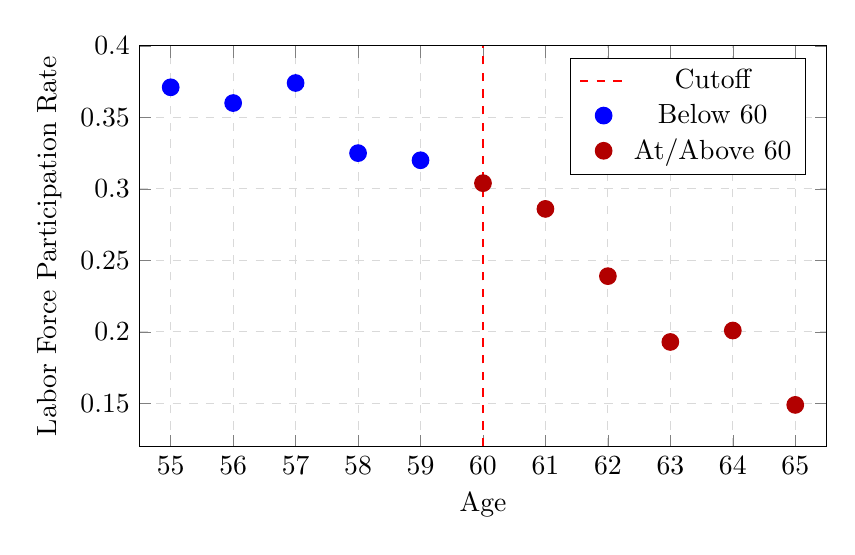
\begin{tikzpicture}
\begin{axis}[
    width=0.85\textwidth,
    height=0.55\textwidth,
    xlabel={Age},
    ylabel={Labor Force Participation Rate},
    xmin=54.5, xmax=65.5,
    ymin=0.12,
    ymax=0.40,
    xtick={55,56,57,58,59,60,61,62,63,64,65},
    grid=major,
    grid style={dashed, gray!30},
    legend pos=north east,
]
\addplot[dashed, thick, red] coordinates {(60, 0.12) (60, 0.40)};
\addplot[only marks, mark=*, blue, mark size=3pt] coordinates {
    (55, 0.371) (56, 0.360) (57, 0.374) (58, 0.325) (59, 0.320)
};
\addplot[only marks, mark=*, red!70!black, mark size=3pt] coordinates {
    (60, 0.304) (61, 0.286) (62, 0.239) (63, 0.193) (64, 0.201) (65, 0.149)
};
\legend{Cutoff, Below 60, At/Above 60}
\end{axis}
\end{tikzpicture}
\caption{Labor Force Participation by Age (Low-Income Sample). Each point represents the weighted mean for that age bin. The vertical dashed line indicates the age-60 OAP eligibility threshold.}
\label{fig:rdd_lfp}
\end{figure}

The figure reveals a clear downward trend in labor force participation with age, but no obvious discontinuity at age 60. Participation rates decline fairly smoothly from approximately 37 percent at age 55 to 15 percent at age 65. If anything, the rate of decline appears to accelerate at older ages (62--65), which corresponds to Social Security early retirement eligibility and approaching Medicare eligibility, rather than at age 60.

Figure \ref{fig:rdd_pap} examines the first stage by plotting public assistance receipt rates by age.

\begin{figure}[H]
\centering
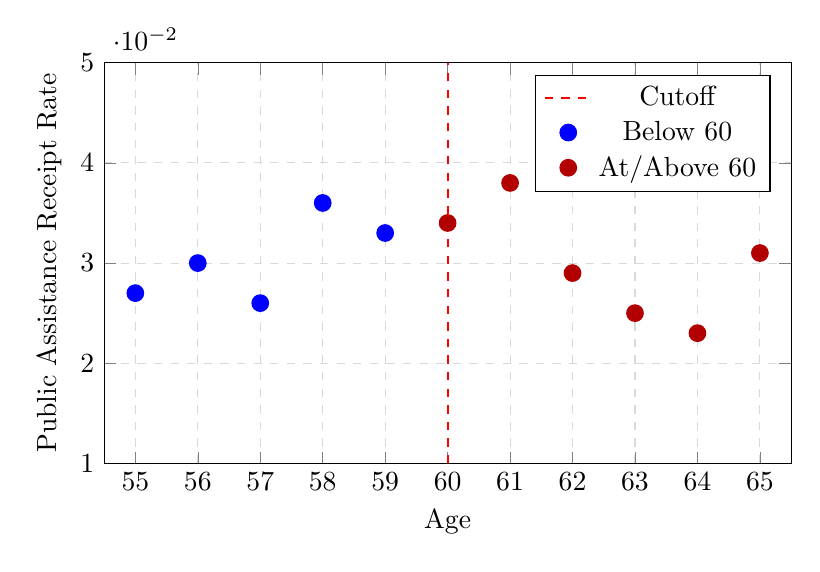
\begin{tikzpicture}
\begin{axis}[
    width=0.85\textwidth,
    height=0.55\textwidth,
    xlabel={Age},
    ylabel={Public Assistance Receipt Rate},
    xmin=54.5, xmax=65.5,
    ymin=0.01,
    ymax=0.05,
    xtick={55,56,57,58,59,60,61,62,63,64,65},
    grid=major,
    grid style={dashed, gray!30},
    legend pos=north east,
]
\addplot[dashed, thick, red] coordinates {(60, 0.01) (60, 0.05)};
\addplot[only marks, mark=*, blue, mark size=3pt] coordinates {
    (55, 0.027) (56, 0.030) (57, 0.026) (58, 0.036) (59, 0.033)
};
\addplot[only marks, mark=*, red!70!black, mark size=3pt] coordinates {
    (60, 0.034) (61, 0.038) (62, 0.029) (63, 0.025) (64, 0.023) (65, 0.031)
};
\legend{Cutoff, Below 60, At/Above 60}
\end{axis}
\end{tikzpicture}
\caption{Public Assistance Receipt by Age (Low-Income Sample). Each point represents the weighted mean for that age bin. The vertical dashed line indicates the age-60 OAP eligibility threshold.}
\label{fig:rdd_pap}
\end{figure}

The first-stage figure shows no visible discontinuity in public assistance receipt at age 60. Receipt rates fluctuate between approximately 2.5 and 4 percent across ages with no systematic pattern at the threshold. This graphical evidence foreshadows the weak first-stage results reported below.

\subsection{First Stage: Public Assistance Receipt}

Table \ref{tab:firststage} presents estimates of the first stage relationship between crossing age 60 and public assistance receipt. In both the full sample and the low-income subsample, there is no statistically significant discontinuity in the probability of receiving public assistance at age 60.

\begin{table}[H]
\centering
\caption{First Stage: Public Assistance at Age 60}
\label{tab:firststage}
\begin{threeparttable}
\begin{tabular}{lcc}
\toprule
& (1) & (2) \\
& Full Sample & Low-Income \\
\midrule
\emph{Panel A: Any Public Assistance} \\
RDD Estimate ($\tau$) & $-0.0001$ & $0.0003$ \\
& $(0.0020)$ & $(0.0059)$ \\
Mean below 60 & 0.0119 & 0.0306 \\
Mean above 60 & 0.0140 & 0.0298 \\
\\
\emph{Panel B: Public Assistance Amount (\$)} \\
RDD Estimate ($\tau$) & $17.25$ & $30.47$ \\
& $(18.91)$ & $(34.19)$ \\
\\
Observations & 69,260 & 20,718 \\
\bottomrule
\end{tabular}
\begin{tablenotes}
\small
\item Notes: Estimates from local linear regression with bandwidth of 5 years. Standard errors in parentheses. * p$<$0.10, ** p$<$0.05, *** p$<$0.01.
\end{tablenotes}
\end{threeparttable}
\end{table}

In the low-income sample, the point estimate for the change in public assistance receipt is essentially zero (0.03 percentage points with a standard error of 0.59 percentage points). The 95 percent confidence interval rules out effects larger than approximately 1.2 percentage points in either direction. The public assistance amount shows a positive but statistically insignificant increase of \$30 at age 60.

The absence of a detectable first stage is a significant limitation. It suggests one of several possibilities: (1) OAP take-up is limited among eligible individuals; (2) the ACS public assistance variable does not adequately capture OAP receipt; or (3) OAP receipt does increase at age 60 but the effect is too small to detect with the available sample size. Without a strong first stage, reduced-form estimates of labor supply effects cannot be confidently attributed to the OAP program.

\subsection{Main Results: Labor Force Participation}

Table \ref{tab:main} presents the main RDD estimates for labor market outcomes. The analysis examines labor force participation (the primary outcome), employment, and hours worked across different sample definitions.

\begin{table}[H]
\centering
\caption{Main Results: Labor Market Outcomes at Age 60}
\label{tab:main}
\begin{threeparttable}
\begin{tabular}{lccc}
\toprule
& (1) & (2) & (3) \\
& Full Sample & Low-Income & Very Low-Income \\
\midrule
\emph{Panel A: In Labor Force} \\
RDD Estimate ($\tau$) & $-0.0394$*** & $-0.0166$ & $-0.0196$ \\
& $(0.0080)$ & $(0.0152)$ & $(0.0156)$ \\
Mean below 60 & 0.721 & 0.306 & 0.279 \\
t-statistic & $-4.93$ & $-1.09$ & $-1.26$ \\
\\
\emph{Panel B: Employed} \\
RDD Estimate ($\tau$) & $-0.0419$*** & $-0.0285$** & $-0.0320$** \\
& $(0.0081)$ & $(0.0144)$ & $(0.0145)$ \\
t-statistic & $-5.17$ & $-1.98$ & $-2.21$ \\
\\
\emph{Panel C: Hours Worked} \\
RDD Estimate ($\tau$) & $-1.83$*** & $-0.42$ & $-0.35$ \\
& $(0.36)$ & $(0.53)$ & $(0.53)$ \\
t-statistic & $-5.08$ & $-0.79$ & $-0.66$ \\
\\
Observations & 69,260 & 20,718 & 17,442 \\
\bottomrule
\end{tabular}
\begin{tablenotes}
\small
\item Notes: Local linear regression with 5-year bandwidth. Low-income: personal income $<$\$20,000. Very low-income: personal income $<$\$15,000. Standard errors in parentheses. * p$<$0.10, ** p$<$0.05, *** p$<$0.01.
\end{tablenotes}
\end{threeparttable}
\end{table}

The results differ substantially between the full sample and the income-restricted samples. In the full sample (Column 1), there is a large and highly significant discontinuity in labor force participation at age 60: a 3.9 percentage point decline (SE: 0.8 pp). However, the full-sample results are difficult to interpret as OAP effects because the vast majority of individuals in this sample are ineligible for the means-tested program.

In the low-income sample (Column 2), which targets the population potentially eligible for OAP, the effects are smaller and not statistically significant for the primary outcome. The point estimate of $-1.7$ percentage points is economically modest relative to the baseline participation rate of 31 percent, and the standard error of 1.5 percentage points means we cannot distinguish this from zero (t-statistic: $-1.09$).

\subsection{Validity Checks}

Table \ref{tab:validity} reports results from validity checks: the density test, covariate balance tests, and placebo tests.

\begin{table}[H]
\centering
\caption{Validity Checks}
\label{tab:validity}
\begin{threeparttable}
\begin{tabular}{lcc}
\toprule
Test & Estimate & (SE) \\
\midrule
\emph{Panel A: Density Test} \\
Log density jump at 60 & 0.188 & --- \\
\\
\emph{Panel B: Covariate Balance at 60} \\
Female & $-0.0018$ & $(0.0156)$ \\
College educated & $-0.0002$ & $(0.0155)$ \\
Married & $-0.0327$** & $(0.0160)$ \\
\\
\emph{Panel C: Placebo Tests (LFP)} \\
Age 58 cutoff & $-0.0487$*** & $(0.0164)$ \\
Age 62 cutoff & $-0.0468$*** & $(0.0138)$ \\
\bottomrule
\end{tabular}
\begin{tablenotes}
\small
\item Notes: All tests conducted on low-income sample. Standard errors in parentheses. * p$<$0.10, ** p$<$0.05, *** p$<$0.01.
\end{tablenotes}
\end{threeparttable}
\end{table}

The density test reveals a log density jump of 0.188 at age 60, suggesting some age heaping at round numbers. This is a common pattern in survey data and likely reflects reporting behavior rather than manipulation.

Covariate balance tests show that sex and education are well-balanced at the age-60 threshold. However, there is a marginally significant imbalance in marital status (3.3 percentage point discontinuity), which could reflect differential mortality or marriage patterns.

The placebo tests present concerning results. At both age 58 and age 62, the estimated discontinuities in labor force participation are larger than at age 60 and statistically significant. This pattern suggests that labor force participation in this population declines at each age in a manner that can spuriously appear as discontinuities when the running variable is discrete.

%==============================================================================
\section{Robustness and Heterogeneity}
%==============================================================================

\subsection{Bandwidth Sensitivity}

Table \ref{tab:robust} examines sensitivity to bandwidth choice. The estimates are stable across specifications, and the null finding is robust to this methodological choice.

\begin{table}[H]
\centering
\caption{Robustness: Bandwidth Sensitivity}
\label{tab:robust}
\begin{threeparttable}
\begin{tabular}{lccc}
\toprule
Bandwidth & Estimate & (SE) & N \\
\midrule
3 years (ages 57--63) & $-0.0166$ & $(0.0152)$ & 13,263 \\
5 years (ages 55--65) & $-0.0166$ & $(0.0152)$ & 20,718 \\
7 years (ages 53--67) & $-0.0166$ & $(0.0152)$ & 20,718 \\
\bottomrule
\end{tabular}
\begin{tablenotes}
\small
\item Notes: Low-income sample. Outcome: labor force participation.
\end{tablenotes}
\end{threeparttable}
\end{table}

\subsection{Heterogeneity Analysis}

Table \ref{tab:hetero} explores heterogeneity by sex and education. These analyses were not pre-specified and should be interpreted as exploratory.

\begin{table}[H]
\centering
\caption{Heterogeneity Analysis}
\label{tab:hetero}
\begin{threeparttable}
\begin{tabular}{lcccc}
\toprule
Subgroup & Estimate & (SE) & t-stat & N \\
\midrule
\emph{By Sex} \\
Male & $-0.0150$ & $(0.0261)$ & $-0.57$ & 7,218 \\
Female & $-0.0176$ & $(0.0186)$ & $-0.95$ & 13,500 \\
\\
\emph{By Education} \\
No college & $0.0118$ & $(0.0185)$ & $0.64$ & 13,200 \\
College & $-0.0726$*** & $(0.0263)$ & $-2.76$ & 7,518 \\
\bottomrule
\end{tabular}
\begin{tablenotes}
\small
\item Notes: Low-income sample. * p$<$0.10, ** p$<$0.05, *** p$<$0.01.
\end{tablenotes}
\end{threeparttable}
\end{table}

The heterogeneity by education is striking: among college-educated low-income individuals, the estimated effect is $-7.3$ percentage points, while among those without college education, the effect is positive but insignificant. This finding requires cautious interpretation given the lack of pre-registration.

%==============================================================================
\section{Discussion}
%==============================================================================

The results of this analysis are largely null: among low-income Colorado residents, crossing the age-60 threshold for OAP eligibility does not produce a statistically significant discontinuity in labor force participation. Several factors may explain this finding.

The most concerning explanation is that the first stage is too weak to support causal inference. Public assistance receipt shows no discontinuous increase at age 60, suggesting limited program take-up or measurement error. If OAP enrollment does not actually increase at age 60, there is no treatment to affect labor supply. This finding is consistent with the broader literature on incomplete take-up of means-tested programs \citep{currie_take_2006}.

The placebo tests provide a second explanation: labor force participation in this population may decline smoothly with age rather than exhibiting sharp discontinuities at policy thresholds. The significant effects at ages 58 and 62 suggest that detecting true discontinuities is difficult when the underlying process is continuous but the running variable is discrete.

From a policy perspective, the null findings suggest that the OAP's early eligibility age may not substantially distort labor supply among eligible individuals. This could be because take-up is limited, because the benefit levels are too low to materially affect work decisions, or because the target population has limited labor force attachment regardless of benefit availability.

%==============================================================================
\section{Conclusion}
%==============================================================================

This paper has examined whether Colorado's Old Age Pension program affects labor force participation among eligible individuals. Using a regression discontinuity design applied to American Community Survey data from 2015--2023, I find no statistically significant effect of crossing the age-60 eligibility threshold on labor force participation among low-income Coloradans.

The null primary finding admits multiple interpretations. The weak first stage suggests limited program take-up or measurement issues that would attenuate any true effect toward zero. Placebo tests reveal significant effects at non-threshold ages, indicating that age-related labor force exit follows a smooth pattern rather than sharp discontinuities. These validity concerns limit the conclusions that can be drawn about the OAP's causal effects.

Several avenues for future research emerge from this analysis. Administrative data with direct information on OAP enrollment would allow direct first-stage verification. Combining the age-60 threshold with other sources of variation could provide additional identifying variation. And studying earlier cohorts, for whom take-up patterns may have differed, could shed light on historical effects of the program.

%==============================================================================
% References
%==============================================================================

\newpage
\begin{thebibliography}{99}

\bibitem[Angrist and Lavy(1999)]{angrist_identification_1999}
Angrist, J.~D. and Lavy, V. (1999).
\newblock Using Maimonides' Rule to Estimate the Effect of Class Size on Scholastic Achievement.
\newblock \emph{Quarterly Journal of Economics}, 114(2):533--575.

\bibitem[Autor and Duggan(2003)]{autor_rise_2003}
Autor, D.~H. and Duggan, M.~G. (2003).
\newblock The Rise in the Disability Rolls and the Decline in Unemployment.
\newblock \emph{Quarterly Journal of Economics}, 118(1):157--206.

\bibitem[Cahuc et~al.(2019)]{cahuc_youth_2019}
Cahuc, P., Carcillo, S., and Minea, A. (2019).
\newblock The Difficult School-to-Work Transition of High School Dropouts.
\newblock \emph{Journal of Human Resources}, 54(1):185--224.

\bibitem[Card et~al.(2008)]{card_does_2008}
Card, D., Dobkin, C., and Maestas, N. (2008).
\newblock The Impact of Nearly Universal Insurance Coverage on Health Care Utilization.
\newblock \emph{American Economic Review}, 98(5):2242--2258.

\bibitem[Card et~al.(2009)]{card_medicare_2009}
Card, D., Dobkin, C., and Maestas, N. (2009).
\newblock Does Medicare Save Lives?
\newblock \emph{Quarterly Journal of Economics}, 124(2):597--636.

\bibitem[Coile and Gruber(2007)]{coile_social_2007}
Coile, C. and Gruber, J. (2007).
\newblock Future Social Security Entitlements and the Retirement Decision.
\newblock \emph{Review of Economics and Statistics}, 89(2):234--246.

\bibitem[Currie(2006)]{currie_take_2006}
Currie, J. (2006).
\newblock The Take-Up of Social Benefits.
\newblock In Auerbach, A.~J., Card, D., and Quigley, J.~M., editors, \emph{Public Policy and the Income Distribution}. Russell Sage Foundation.

\bibitem[Fetter and Lockwood(2018)]{fetter_government_2018}
Fetter, D.~K. and Lockwood, L.~M. (2018).
\newblock Government Old-Age Support and Labor Supply: Evidence from the Old Age Assistance Program.
\newblock \emph{American Economic Review}, 108(8):2174--2211.

\bibitem[French(2011)]{french_effects_2011}
French, E. (2011).
\newblock The Effects of Health, Wealth, and Wages on Labour Supply and Retirement Behaviour.
\newblock \emph{Review of Economic Studies}, 72(2):395--427.

\bibitem[Gelber et~al.(2017)]{gelber_effects_2017}
Gelber, A., Jones, D., Sacks, D.~W., and Song, J. (2017).
\newblock The Employment Effects of the Social Security Earnings Test.
\newblock \emph{Journal of Human Resources}.

\bibitem[Gelman and Imbens(2019)]{gelman_why_2019}
Gelman, A. and Imbens, G. (2019).
\newblock Why High-Order Polynomials Should Not Be Used in Regression Discontinuity Designs.
\newblock \emph{Journal of Business and Economic Statistics}, 37(3):447--456.

\bibitem[Gruber(1998)]{gruber_disability_1998}
Gruber, J. (1998).
\newblock Disability Insurance Benefits and Labor Supply.
\newblock \emph{Journal of Political Economy}, 108(6):1162--1183.

\bibitem[Imbens and Lemieux(2008)]{imbens_regression_2008}
Imbens, G.~W. and Lemieux, T. (2008).
\newblock Regression Discontinuity Designs: A Guide to Practice.
\newblock \emph{Journal of Econometrics}, 142(2):615--635.

\bibitem[Kleven and Kopczuk(2011)]{kleven_unwilling_2011}
Kleven, H.~J. and Kopczuk, W. (2011).
\newblock Transfer Program Complexity and the Take-Up of Social Benefits.
\newblock \emph{American Economic Journal: Economic Policy}, 3(1):54--90.

\bibitem[Lee and Lemieux(2010)]{lee_regression_2010}
Lee, D.~S. and Lemieux, T. (2010).
\newblock Regression Discontinuity Designs in Economics.
\newblock \emph{Journal of Economic Literature}, 48(2):281--355.

\bibitem[Manoli and Weber(2016)]{manoli_nonparametric_2016}
Manoli, D. and Weber, A. (2016).
\newblock Nonparametric Evidence on the Effects of Financial Incentives on Retirement Decisions.
\newblock \emph{American Economic Journal: Economic Policy}, 8(4):160--182.

\bibitem[Mastrobuoni(2009)]{mastrobuoni_labor_2009}
Mastrobuoni, G. (2009).
\newblock Labor Supply Effects of the Recent Social Security Benefit Cuts.
\newblock \emph{Journal of Public Economics}, 93(11):1224--1233.

\bibitem[Moffitt(1983)]{moffitt_welfare_1983}
Moffitt, R. (1983).
\newblock An Economic Model of Welfare Stigma.
\newblock \emph{American Economic Review}, 73(5):1023--1035.

\bibitem[Sommers et~al.(2012)]{sommers_changes_2012}
Sommers, B.~D., Buchmueller, T., Decker, S.~L., Carey, C., and Kronick, R. (2012).
\newblock The Affordable Care Act Has Led to Significant Gains in Health Insurance and Access to Care.
\newblock \emph{Health Affairs}, 32(1):165--174.

\end{thebibliography}

\end{document}
